\documentclass[]{article}
\usepackage{atlasphysics}
% Nice maths macros
\usepackage{amsmath}
% Units
\usepackage{siunitx}
% Figures and floats
\usepackage{graphicx,subfigure,float}

% Graphics folider
\graphicspath{{figures/}}

% Scientific notation
% http://www.tapdancinggoats.com/easy-scientific-notation-in-latex.htm
\providecommand{\e}[1]{\ensuremath{\times 10^{#1}}}
% Differential Operator
\renewcommand{\d}[1]{\ensuremath{\,\operatorname{d}\!{#1}}}
% Absolute value
\renewcommand{\mod}[1]{\ensuremath{\lvert {#1} \rvert}}
% Airys functions Ai(x) and Bi(x)
\newcommand{\Ai}[1]{\ensuremath{\operatorname{Ai}({#1})}}
\newcommand{\Bi}[1]{\ensuremath{\operatorname{Bi}({#1})}}

\begin{document}

\title{Masses of S-State Mesons - Notes}
\author{Alex Pearce}
\date{\today}
\maketitle


\begin{abstract}
Morbi ac commodo nulla. In condimentum orci id nisl volutpat bibendum. Quisque commodo hendrerit lorem quis egestas. Maecenas quis tortor arcu. Vivamus rutrum nunc non neque consectetur quis placerat neque lobortis. Nam vestibulum, arcu sodales feugiat consectetur, nisl orci bibendum elit, eu euismod magna sapien ut.
\end{abstract}

\section{Some Formulae}

Radial Schr\"{o}dinger equation for two particles interacting via potential $V(r)$ with a reduced mass $m$:
\[
-\frac{\hbar^{2}}{2m}\left (
	\frac{1}{r^{2}} \frac{\d{}}{\d{r}} \left (
		r^{2} \frac{\d{\psi}}{\d{r}}
	\right )
	- \frac{\ell(\ell+1)}{r^{2}}\psi
\right )
+ V(r)\psi = E\psi.
\]
with linear potential $V(r) = kr$ such that $\partial V / \partial r = k$ is constant.

Applying the boundary conditions and implementing change of variable $u = r\psi$, u satisfies

\[
-\frac{\hbar^{2}}{2m}\left (
	u''
	- \frac{\ell(\ell+1)}{r^{2}}u
\right )
+ V(r)u = Eu.
\]

As we are only concerned with $\ell = 0$ we perform another change or variable $r = ax + b$, with $a = \sqrt[3]{2mk/\hbar^{2}}$ and $b = E/k$, to bring us to

\[
\frac{\d{y}}{\d{x}} - xy = 0.
\]

This is Airy's equation and has been is well studied. It is analytically solvable with solutions of the form
\[
y(x) = c\Ai{x} + d\Bi{x},
\]
where $\Ai{x}$ and $\Bi{x}$ are the Airy functions. As $\Bi{x}$ has a singularity at $x=\infty$ it does not satisfy the boundary conditions and so $d=0$.

The first Airy function $\Ai{x}$ may be approximated for small $\mod{x}$ as
\[
\Ai{x} = 0.3550280538f(x) - 0.2588194037g(x),
\]
where $f(x)$ and $g(x)$ are infinite series given by
\begin{align*}
f(x) &= 1 + \frac{1}{3!}x^{3} + \frac{1\times4}{6!}x^{6} + \frac{1\times4\times{7}}{9!}x^{9} + \dotsb,\\
g(x) &= x + \frac{2}{4!}x^{4} + \frac{2\times5}{7!}x^{7} + \frac{2\times5\times{8}}{10!}x^{10} + \dotsb.
\end{align*}

After some arithmetic, it can be shown that the two infinite series may be represented recursively. The $n$th term in each series may then be given by
\begin{align*}
f_{n}(x) &= \frac{f_{n-1}(x)}{(3n^{2} - n)} \frac{x^{3}}{3},\\ 
g_{n}(x) &= \frac{g_{n-1}(x)}{(3n^{2} + n)} \frac{x^{3}}{3},
\end{align*}

for $f_{0}(x) = 1$ and $g_{0}(x) = x$. This should save considerable computation time as the highest power of $x$ we need to compute is $x^{3}$.

For larger $\mod{x}$, we may use the alternative approximations
\[
\Ai{x} \approx \frac{1}{2}\pi^{-1/2}x^{-1/4}e^{-\zeta} \sum\limits_{k=0} (-1)^{k}c_{k}\zeta^{-k},
\]
and
\[
\Ai{-x} \approx \pi^{-1/2}x^{-1/4}\left (
	\sin{(\zeta + \frac{\pi}{4})}\sum\limits_{k=0}(-1)^{k}c_{2k}\zeta^{-2k} -
	\cos{(\zeta + \frac{\pi}{4})}\sum\limits_{k=0}(-1)^{k}c_{2k+1}\zeta^{-(2k+1)}
\right ),
\]
where
\[
c_{k} = \frac{(2k+1)(2k+3)\dotsb(6k-1)}{216^{k}k!}, \quad c_{0} = 1
\]
and
\[
\zeta = \frac{2}{3}x^{3/2}.
\]
This is the Chebyshev expansion of Airy's function $\Ai{x}$~\cite{ref:agil}. Wolfram Alpha can plot $c_{k}$ with
\begin{verbatim}
(Gamma(3 k+1/2))/(54^k k! Gamma(k+1/2)) from 0 to 7
\end{verbatim}

To first order we have
\[
\Ai{x} = \begin{cases}
	\frac{1}{2}\pi^{-1/2}\mod{x}^{-1/4}\exp{(-\zeta)} & x > 0\\
	\pi^{-1/2}\mod{x}^{-1/4} \left (
		\zeta^{0}\sin{(\zeta + \frac{\pi}{4})} - c_{1}\zeta^{-1}\cos{(\zeta + \frac{\pi}{4})}
	\right ) & x < 0
\end{cases}
\]
where $c_{1} = 15/216$.

The problem is then finding the zeros of $\Ai{x}$.

\subsection{Roots of $\Ai{x}$}

The second boundary conditions requires that $u = 0$ at $r = 0$, that is $y = 0$ at $x = -b/a$, where
\[
a = \sqrt[3]{\frac{2mk}{\hbar^{2}}},\quad b = \frac{E}{k}
\quad\Rightarrow\quad x = -\frac{E}{k}\sqrt[3]{\frac{\hbar^{2}}{2mk}}.
\]
So the $n$th energy level of the two quark system is $$E_{n} = -\frac{x_{n}k}{\sqrt[3]{2mk/\hbar^{2}}}$$ where $x_{n}$ is the $n$th root of $\Ai{x}$. This is dimensionally correct: $a$ has dimensions of $\si{\metre}$ and $k$ has dimensions of $\si{\joule\per\metre}$, making $x$ dimensionless and $E$ in dimensions of $\si{\joule}$.


\subsection{Finding the Quark Masses}

The formula for the the mass of a meson with quantum numbers $n$ and $l$ is $$M_{n,l} = 2m_{q} + E_{n,l},$$ where $m_{q}$ is the quark mass, and $E_{n,l}$ is the binding energy obtained from the Schr\"{o}dinger equation.

We may then use the experimental meson masses to find the  proportionality constant $k$ and therefore the quark mass $m_{q}$.

\begin{table}[H]
	\begin{center}
		\subtable[Charm Mesons $\ccbar$] {
		\begin{tabular}{ c | c c c }
			%\multicolumn{4}{c}{Charm Mesons}\\
			$n$ & $\ell = 0$ & $\ell = 1$ & $\ell = 2$ \\ \hline
			1 & 3.10 & 3.50 & 3.77 \\
			2 & 3.69 & & \\
			3 & 4.04 & & \\
		\end{tabular}
		%\caption{Charm Mesons $\ccbar$}
		\centering
		}
		\quad % spacing
		\subtable[Bottom Mesons $\bbbar$] {
			\begin{tabular}{ c | c c c c }
				%\multicolumn{4}{c}{Bottom Mesons}\\
				$n$ & $\ell = 0$ & $\ell = 1$ & $\ell = 2$\\ \hline
				1 & 9.46 & 9.9\\
				2 & 10.02 & 10.02\\
				3 & 10.35 &\\
				4 & 10.57 &\\
				5 & 10.86 &\\
				6 & 11.02 &\\
			\end{tabular}
			\centering
		}    
		\caption{Meson Masses in \GeV.}
		\label{tab:mesonmasses}
	\end{center}  
\end{table}

By plotting these experimentally obtained meson masses $M_{n,0}$ against the numerical binding energies, we may find the potential constants $k$ and the quark masses ($m_{c}$ and $m_{b}$) by the slope and intercept respectively.


\section{Data}

The script gives a charm mass of $m_{c} = 1.2138\GeV$ and a bottom mass of $m_{b} = 4.5056\GeV$ (via the fact that the intercept is $2m_{q}$). The slopes were $0.29689$ for the charm and $0.23004$ for the bottom. We may extract the $k$ values using
$$M_{n,0} = 2m_{q} - x_{n}\left(\frac{k^{2}\hbar^{2}}{2m}\right)^{1/3} = 2m_{q} - \alpha x_{n}.$$
Then, $k$ may be expressed with respect to the slope $\alpha$ as
$$k_{q} = \pm\sqrt{\frac{2m\alpha_{q}^{3}}{\hbar^{2}}}.$$
This gives values of $k_{c} = \num{3.10681e11}\si{\joule\per\metre}$ and $k_{b} = \num{4.08246e11}\si{\joule\per\metre}$.


\section{Figures}\label{sec:figures}

\begin{figure}[H]
	\hspace*{-0.15\textwidth}
	\centering
	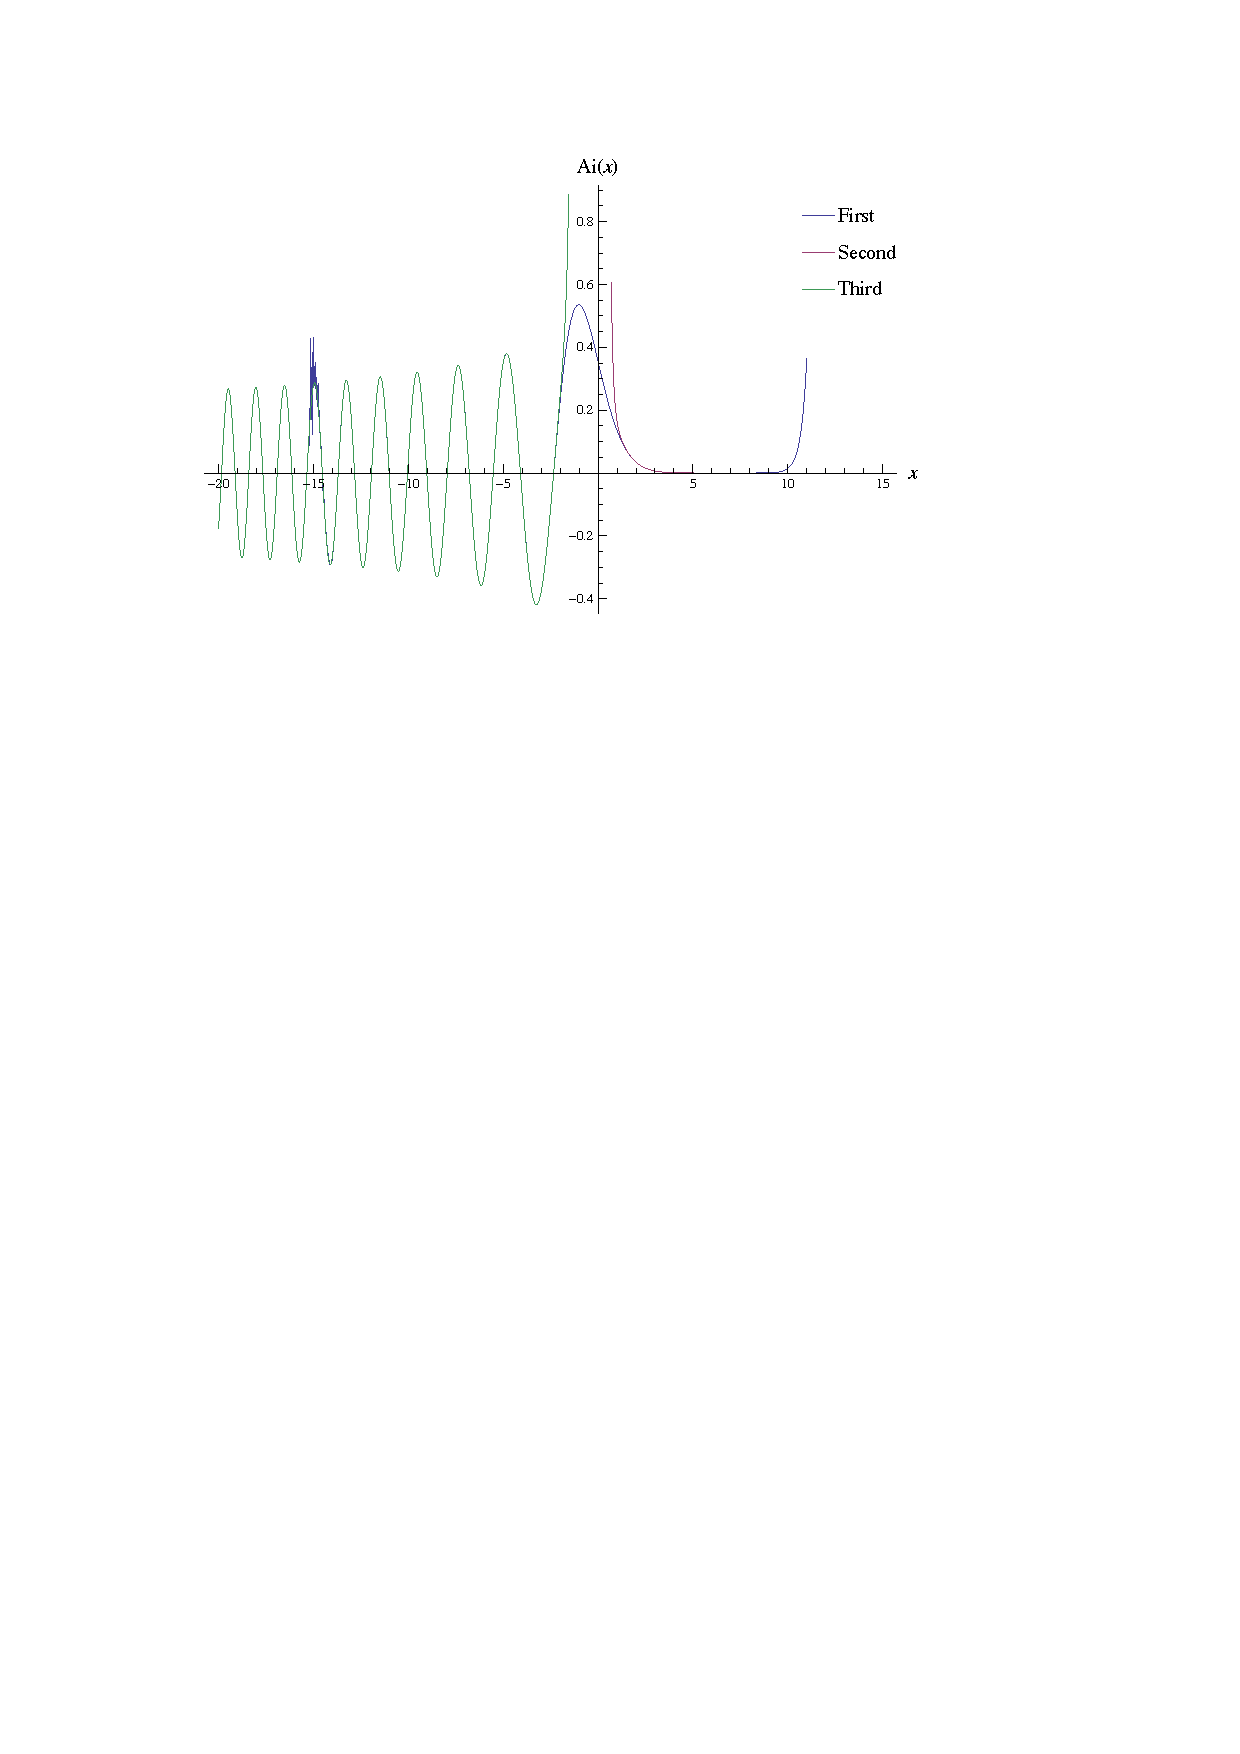
\includegraphics[scale=1.3]{approximations}
	\caption{Approximations!}
	\label{fig:data}
\end{figure}

\begin{figure}[H]
	\hspace*{-0.15\textwidth}
	\centering
	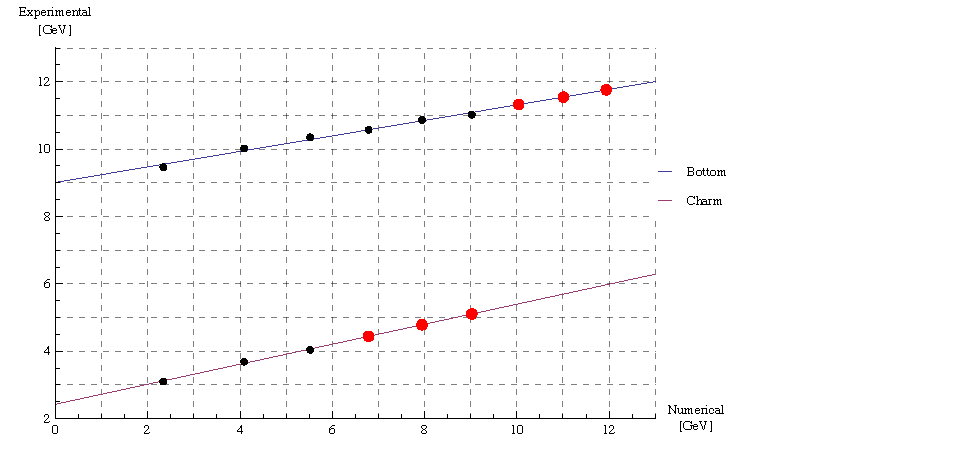
\includegraphics[scale=1.3]{experimental-numerical}
	\caption{Data!}
	\label{fig:data}
\end{figure}

\begin{thebibliography}{9}
	\bibitem{ref:gjdaniell}
  G. J. Daniell,
  \emph{PHYS6017 Course Notes},
  University of Southampton, Southampton, UK,
  2011.
  
	\bibitem{ref:agil}
  A. Gil, J. Segura and N. M. Temme,
  \emph{Numerical Methods for Special Functions},
  Society for Industrial and Applied Mathematics, Philadelphia PA, USA,
  $1$st Edition,
  2007.
  
  \bibitem{ref:nr}
  W. H. Press et al.,
  \emph{Numerical Recipes: The Art of Scientific Computing},
  Cambridge University Press, Cambridge, UK,
  $3$rd Edition,
  2007
  
\end{thebibliography}

\end{document}